% https://blog.kokanovic.org/performance-analysis-of-dlibs-cnn-face-detection/

\chapter{Mérések}
\label{sec:meresek}

Ebben a fejezetben a „face-recognition” könyvtár gyorsaságát vizsgáltam. A precizitást a „face-recognition” garantálja, 99,38\%-os pontosságot ért el a „Faces in the Wild benchmark”-on \cite{artc31}. Az etorobotikai kísérletek szempontjából a pontossághoz tartozik az, hogy a robot adekvátan reaktív, vagyis megfelelő sebességgel reagál az ingerekre (jelen esetben az arc látványára), illetve az arc orientációja sem okoz problémát. A feldolgozás sebességére optimalizáltam az algoritmus kialakításakor, mert ezzel tudtam a legtöbb javulást elérni felhasználói élmény szempontjából. A teljesítmény kiértékelésekor a sebességre, felbontásra, orientációra koncentráltam. Kettő féle mérést implementáltam. Az első mérésben a kép minőségének hatását vizsgálom a feldolgozás sebességében. Különböző felbontású képeken mérem, mennyi ideig tart egy arc feldolgozása. A másodikban egy arc orientációjának hatását vizsgálom a feldolgozási folyamat során. A mérések egyenként több képből állnak és mindegyik képen 6 különböző tesztet futtatok.
\begin{enumerate}
    \item \emph{Arcok lokalizálása:} betöltött képen méri mennyi idő alatt találja meg az arcot vagy arcokat;
    \item \emph{Arcvonások megkeresése:} a betöltött képen egy arc helyének megtalálása után méri az arcvonások felismerésének idejét;
    \item \emph{Arc „enkódolása” a helyekből:} a betöltött képen egy arc helyének megtalálása után méri az arc „enkódolássá” való alakítását
    \item \emph{Arc „enkódolása” kép formátumból:} a kép betöltése után méri az „enkódolássá” alakítás idejét
    \item \emph{Arc felismerése:} kép betöltése és az arc „enkódolása” után méri, hogy mennyi idő amíg az arcot az előre betöltött mintával összehasonlítja és megállapítja egyezésüket
    \item \emph{Felismert arc elmentése:} méri, hogy mennyi idő képre rárajzolni az arcot jelölő téglalapot és nevet
\end{enumerate}

A mérések elvégzéséhez a „face-recognition” könyvtár készítője által írt „benchmark”-ot használom, illetve ezt bővítettem ki a szükséges módosításokkal.\footnote{\url{https://github.com/ageitgey/face_recognition/blob/master/examples/benchmark.py}} A Python timeit\footnote{Python timeit dokumentáció: \url{https://docs.python.org/3/library/timeit.html}} könyvtárát használom, a 6 különböző teszt mindegyike képenként 10-szer fut és számol autómatizáltan átlagolt futási időt. A képeket a dolgozat mellékletében, a használt kódot a feltöltött ROS csomagban mellékeltem.

A teszteket egy processzor magon futtattam az alábbi környezetben:
\begin{itemize}
    \item[] \emph{Hardver}
    \begin{itemize}
        \item[$\blacksquare$] \emph{Processzor:} \verb|Intel® Core™ i5-6300U CPU @ 2.40GHz × 4|
        \item[$\blacksquare$] \emph{Memória:} \verb|16GB DDDR4|
        \item[$\blacksquare$] \emph{Grafikus vezérlő:} \verb|Mesa Intel® HD Graphics 520 (SKL GT2)|
    \end{itemize}
    \item[] \emph{Szoftver}
    \begin{itemize}
        \item[$\blacksquare$] \emph{Operációs rendszer:} \verb|Ubuntu 20.04.5 LTS; 64 bit|
        \item[$\blacksquare$] \emph{Python verzió:} \verb|3.8.10|
        \item[$\blacksquare$] \emph{face-recognition verzió:} \verb|1.3.0|
        \item[$\blacksquare$] \emph{ROS verzió:} \verb|ROS Melodic|
        \item[$\blacksquare$] \emph{opencv-python verzió:} \verb|4.6.0.66|
    \end{itemize}
\end{itemize}

A tesztek során használt képek felbontása 16:9-es képarányt követve:
\begin{table}[!ht]
	\footnotesize
	\centering
	\begin{tabular}{ l c c }
		\toprule
		Jelölés & Felbontás \\
		\midrule
		240p &  426x240 Pixel\\
		480p &  854x480 Pixel\\
        720p &  1280x720 Pixel\\
        1080p &  1920x1080 Pixel\\
		\bottomrule
	\end{tabular}
	\caption{Vizsgált felbontáso.}
	\label{tab:TabularExample}
\end{table}

\clearpage
\section{Felbontás teszt}
% https://github.com/ageitgey/face_recognition/tree/master/examples
A kép, amivel összehasonlítom a beolvasott arcokat (\refstruc{fig:felbontasteszt}) a legjobb minőségű a választott képek közül \verb|1080p| felbontással, aminek a feldolgozása külön történik a tesztek futását megelőzően, nem befolyásolja a lényeges programkód futásának idejét.

%\begin{figure}[!ht]
%	\centering
%	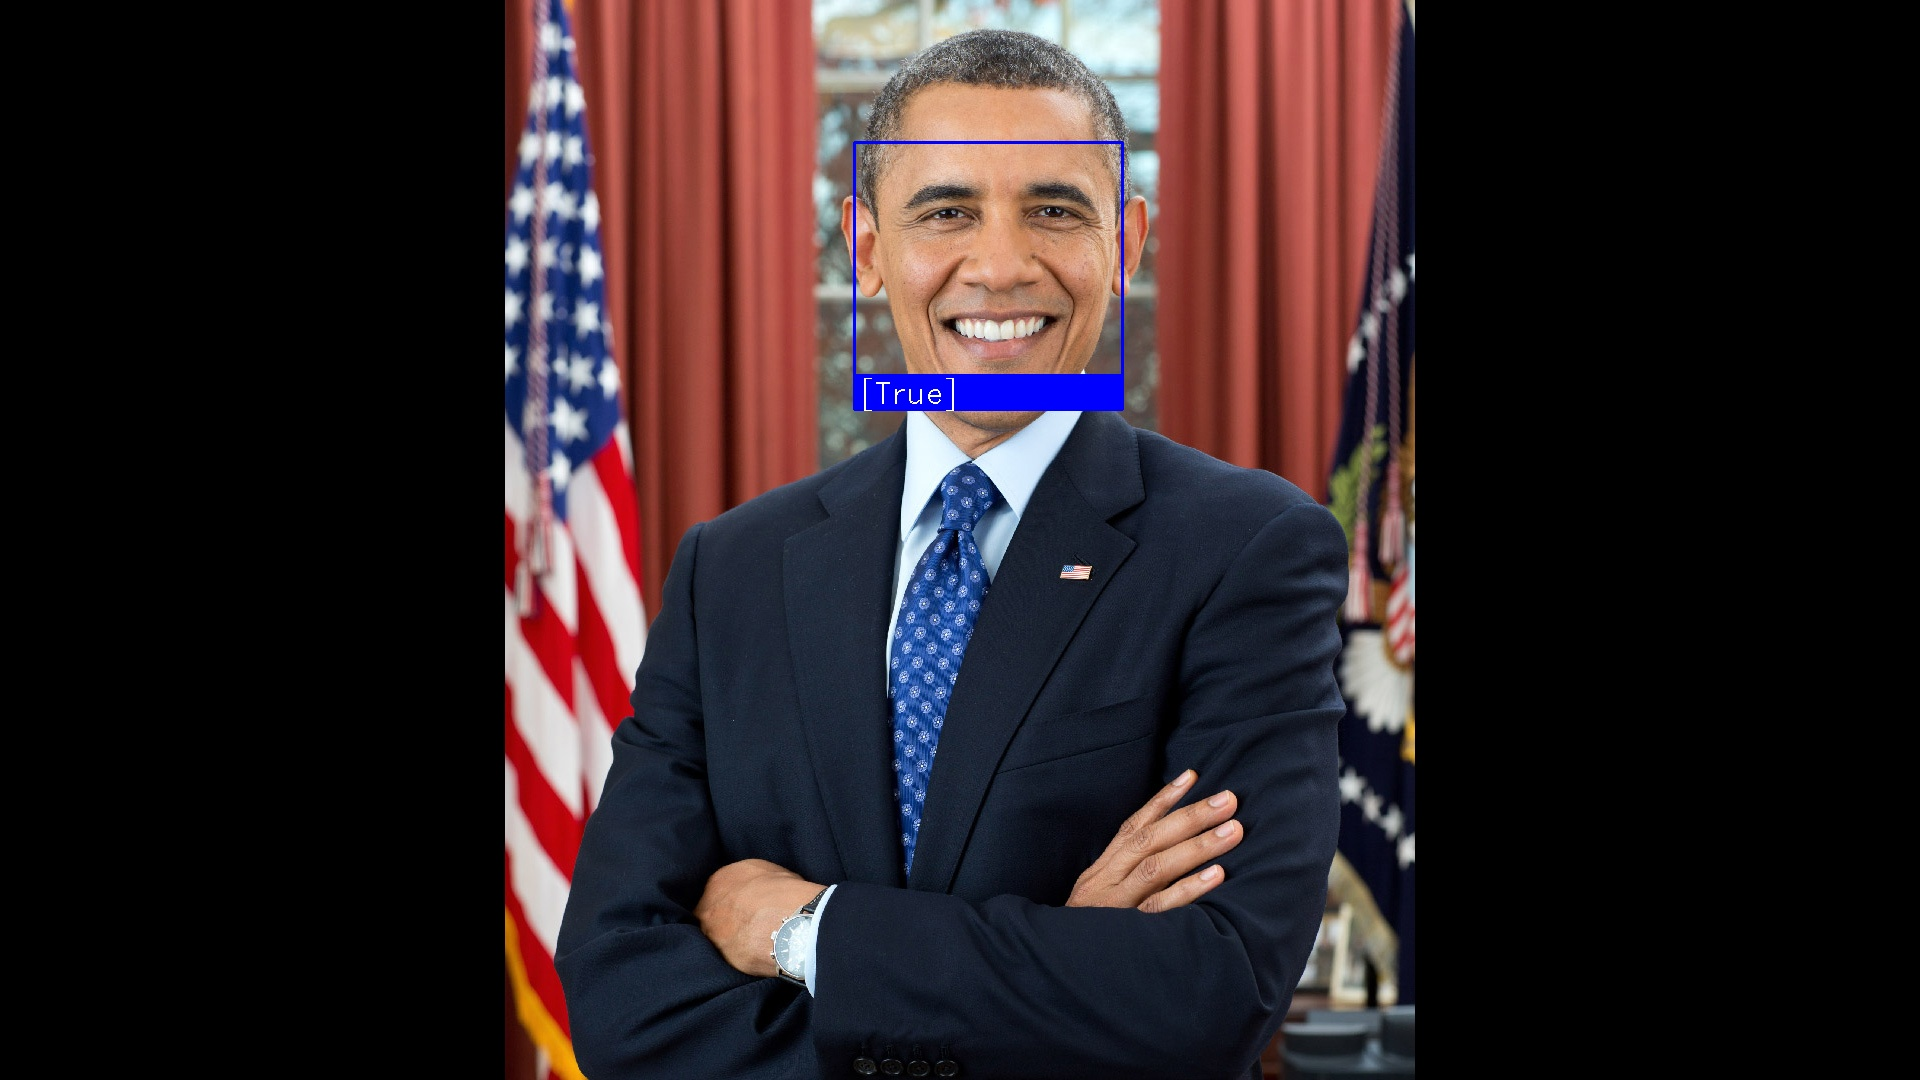
\includegraphics[width=60mm, keepaspectratio]{03_images/obama/o-obama-1080p.jpg}
%	\caption[Minta kép, a felbontás teszteléséhez]{Minta kép, a felbontás teszteléséhez\cite{artc_gold}.}
%	\label{fig:ob_test}
%\end{figure}
%\footnotetext{kép forrása: \url{https://github.com/ageitgey/face_recognition/blob/master/examples/obama-720p.jpg}}

Az \refstruc{fig:res_graphs} mutatja a mérések eredményét. A bal felső grafikonról leolvasható, hogy az arcok helyének megtalálása annál több időt vesz igénybe minél jobb minőségű a kép. Nagyobb felbontás több képpontot jelent, azaz több adatot, ami értelemszerűen nagyobb számítási kapacitást igényel. Mellette az „Enkódolás képből” grafikon a képből az arc „enkódolásának” kinyeréséhez szükséges időt mutatja be. A „Arcvonások” grafikon az arcvonások számosítása során eltelt időt ábrázolja. Az arcok „enkódolását” úgy is ki lehet nyerni a képekből, ha először lefuttatjuk az arcok helyeinek megkeresését, és aztán a helyeket tartalmazó listát is átadjuk az arcokat „enkódoló” függvény számára. Ennek a futásidejét a „Encodings from locations” grafikon mutatja be. Az ábrákból levonható következtetés, hogy amit befolyásol a kép felbontása, az az arcok helyének megtalálása. A két baloldali grafikonból jól látható, hogy amikor már előzetesen megkerestük az arcok helyét, a nagyobb felbontás nem eredményezett láthatóan több futásidőt. A teszt eredeti kimenete a mellékletekben megtalálható(\ref{lst:res_mel}).
\begin{figure}[!ht]
	\centering
	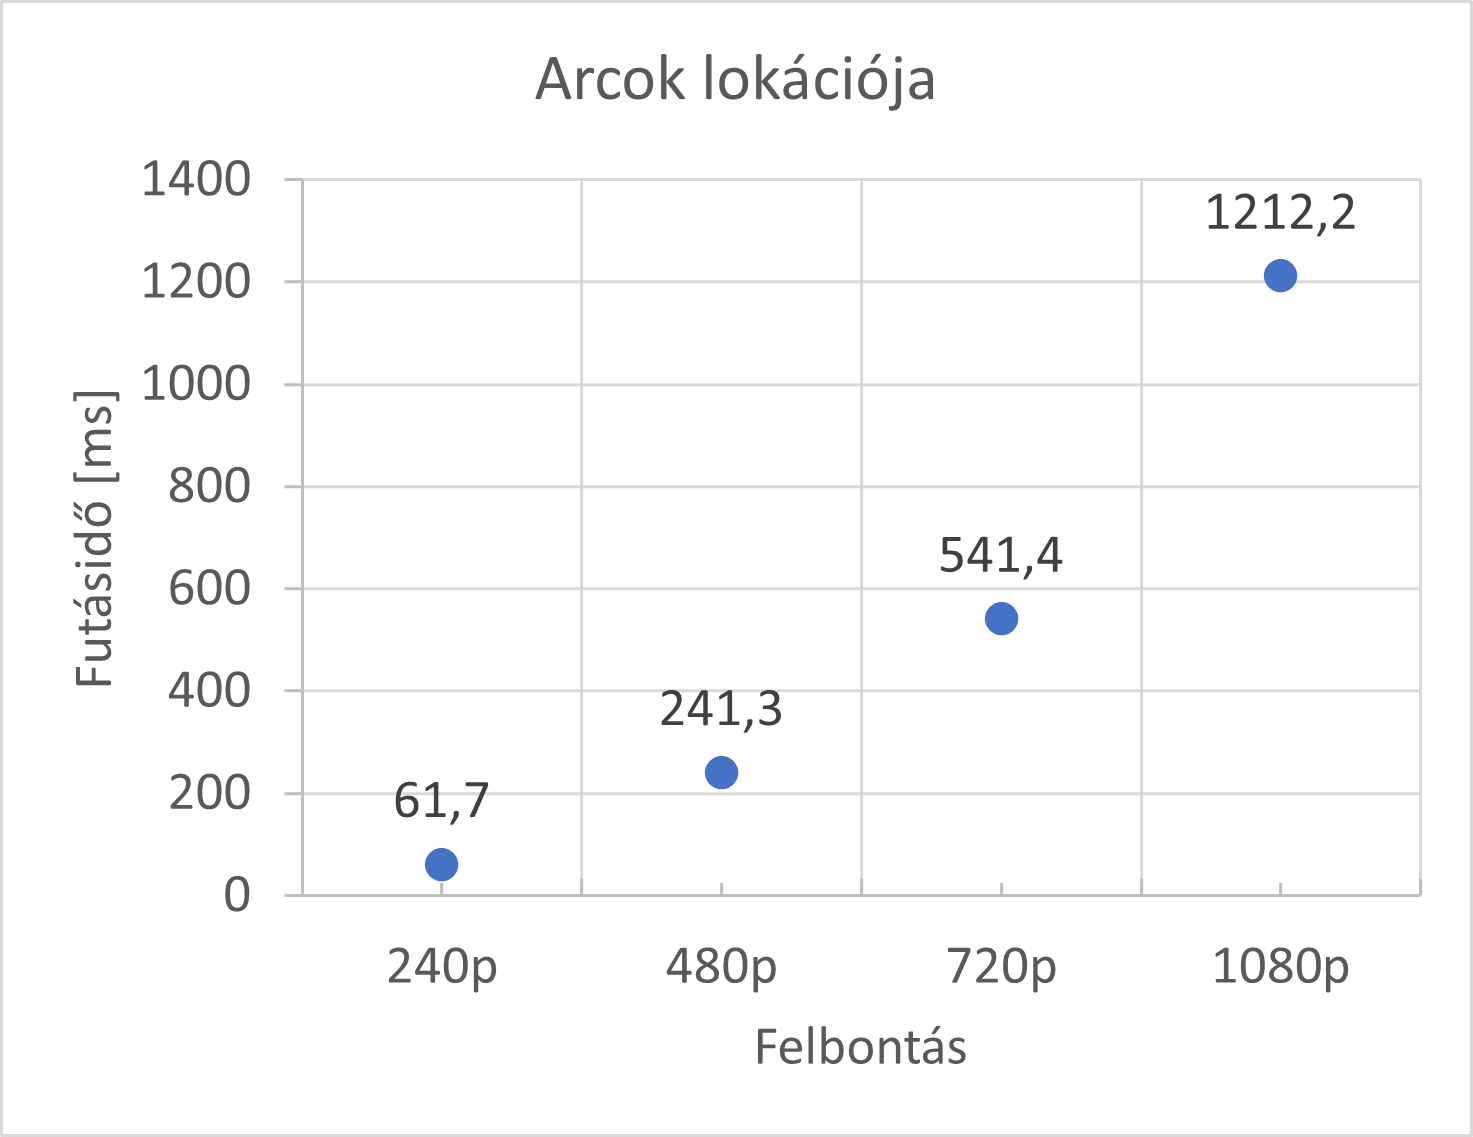
\includegraphics[width=67mm, keepaspectratio]{03_images/graph2/mennyiseg1.png}\hspace{1cm}
	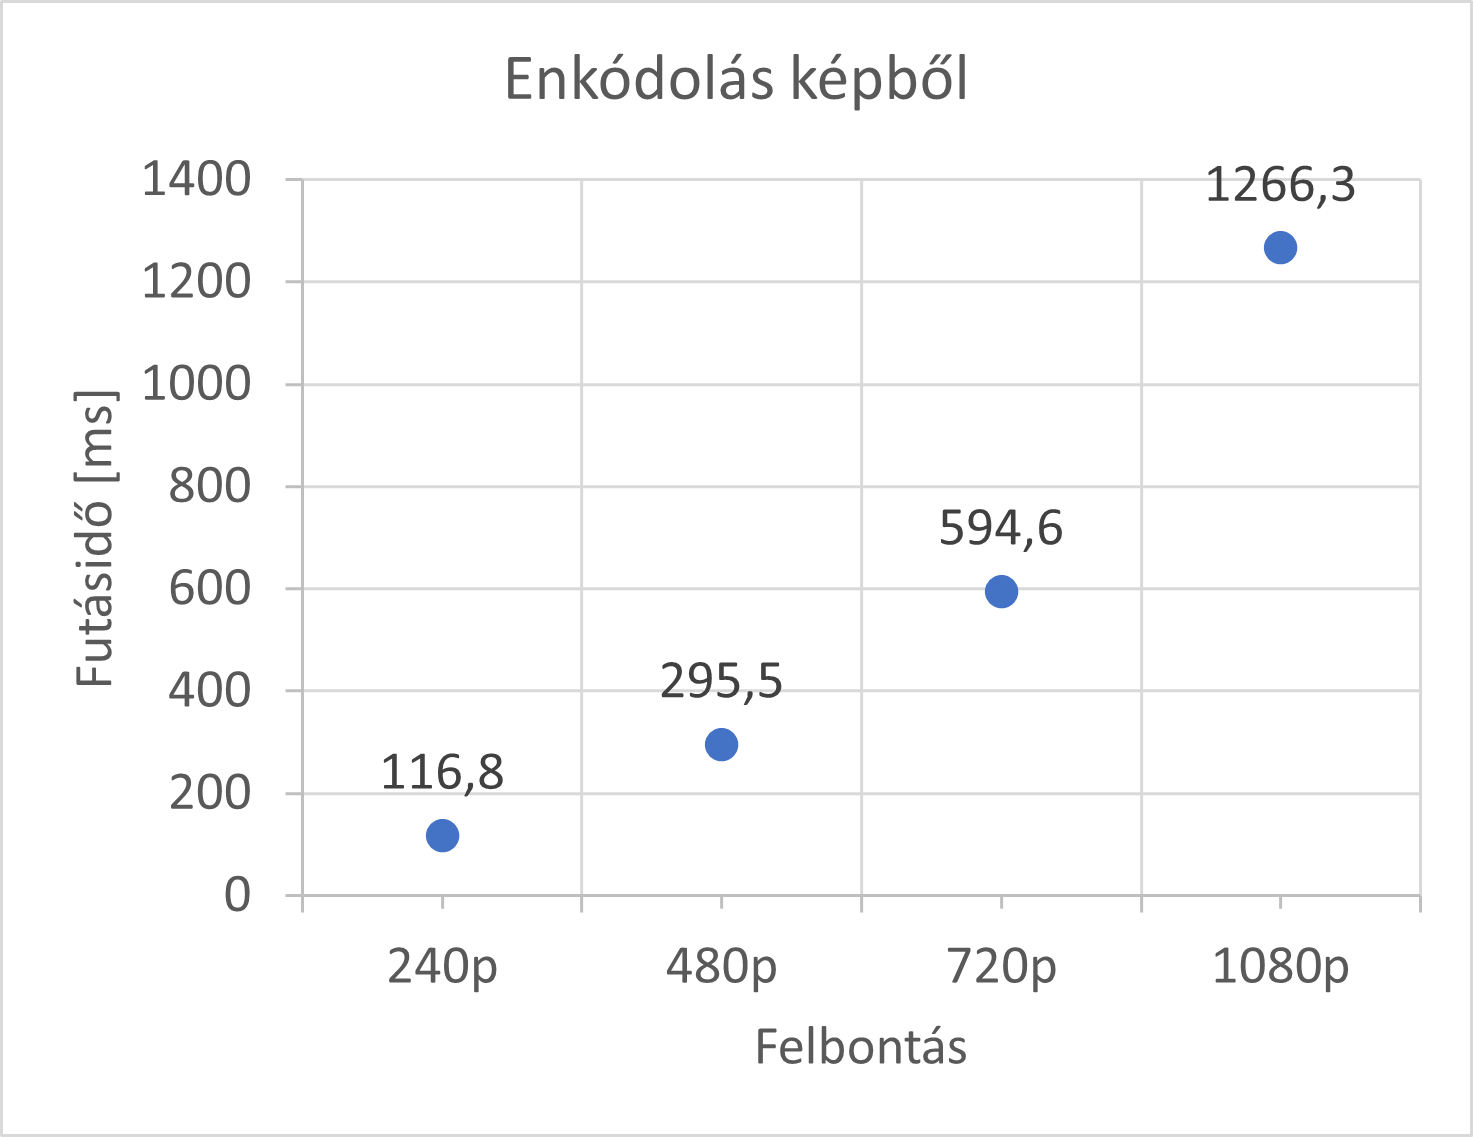
\includegraphics[width=67mm, keepaspectratio]{03_images/graph2/mennyiseg12.png}\\\vspace{5mm}
	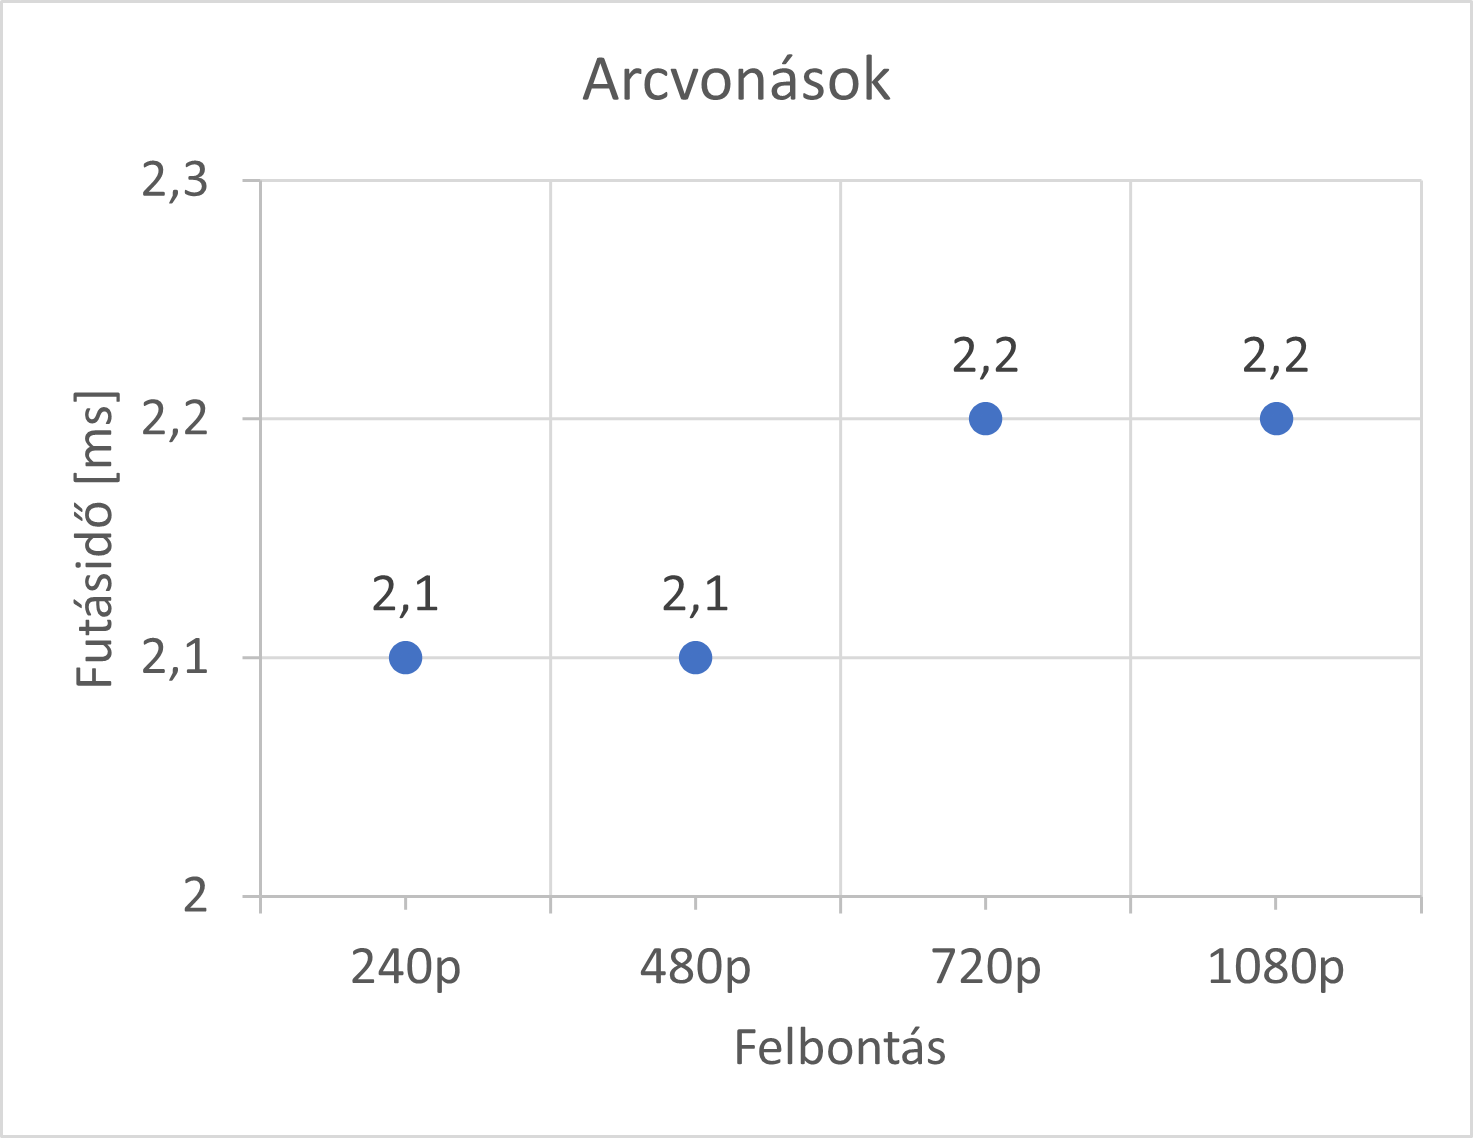
\includegraphics[width=67mm, keepaspectratio]{03_images/graph2/mennyiseg123.png}\hspace{1cm}
	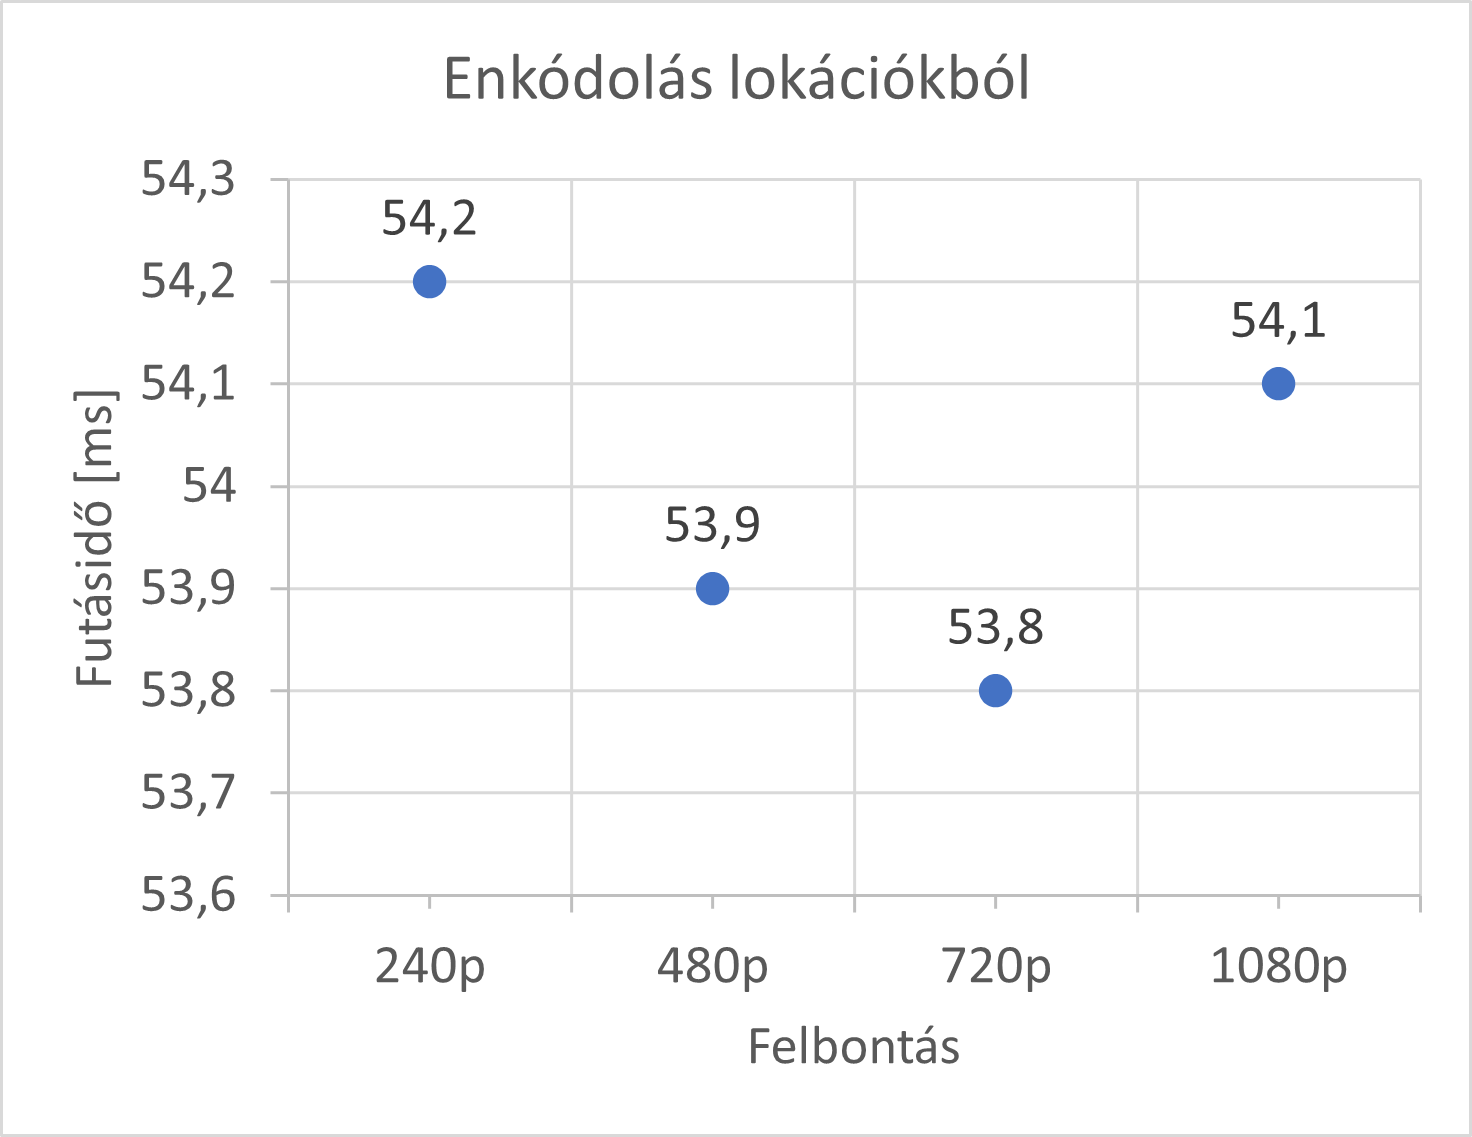
\includegraphics[width=67mm, keepaspectratio]{03_images/graph2/mennyiseg1234.png}
	\caption{Grafikonok a felbontás teszt eredményeiről.}
	\label{fig:res_graphs}
\end{figure}



 \clearpage
\section{Orientáció teszt}
% https://fei.edu.br/~cet/facedatabase.html
Valós alkalmazásban gyakran előfordulhat, hogy az emberek nem néznek bele frontálisan a robot kamerájába, ezért szükséges, hogy a szoftver képes legyen különböző orientációkban is felismerni arcokat. Ebben a mérésben a „FEI Face Database”\cite{artc41}-ből vett képeket elemeztem. Az mellékletben található \refstruc{fig:ori_test} bemutatja, hogy széles horizontálisan változó fej orientációs spektrumon képes az algoritmus arra, hogy felismerjen emberi arcokat.

A mérés során lefuttatott tesztek eredménye a mellékletben található: \ref{lst:ori_mel}. A kapott adatok szemléltetésére készítettem a lenti grafikonokat (\refstruc{fig:ori_graphs}). A minta arcnak, amihez hasonlítottam a különböző képeket egy olyat válsztottam, melyen a személy a kamerába néz. A vizsgált képek mérete és felbontása megegyezik. A grafikonokról megállapítható, hogy az elforgatott arcok nem befolyásolják se az arc helyének megkeresésére fordított időt, se az „enkódolásra” fordított időt. 
\begin{figure}[!ht]
	\centering
	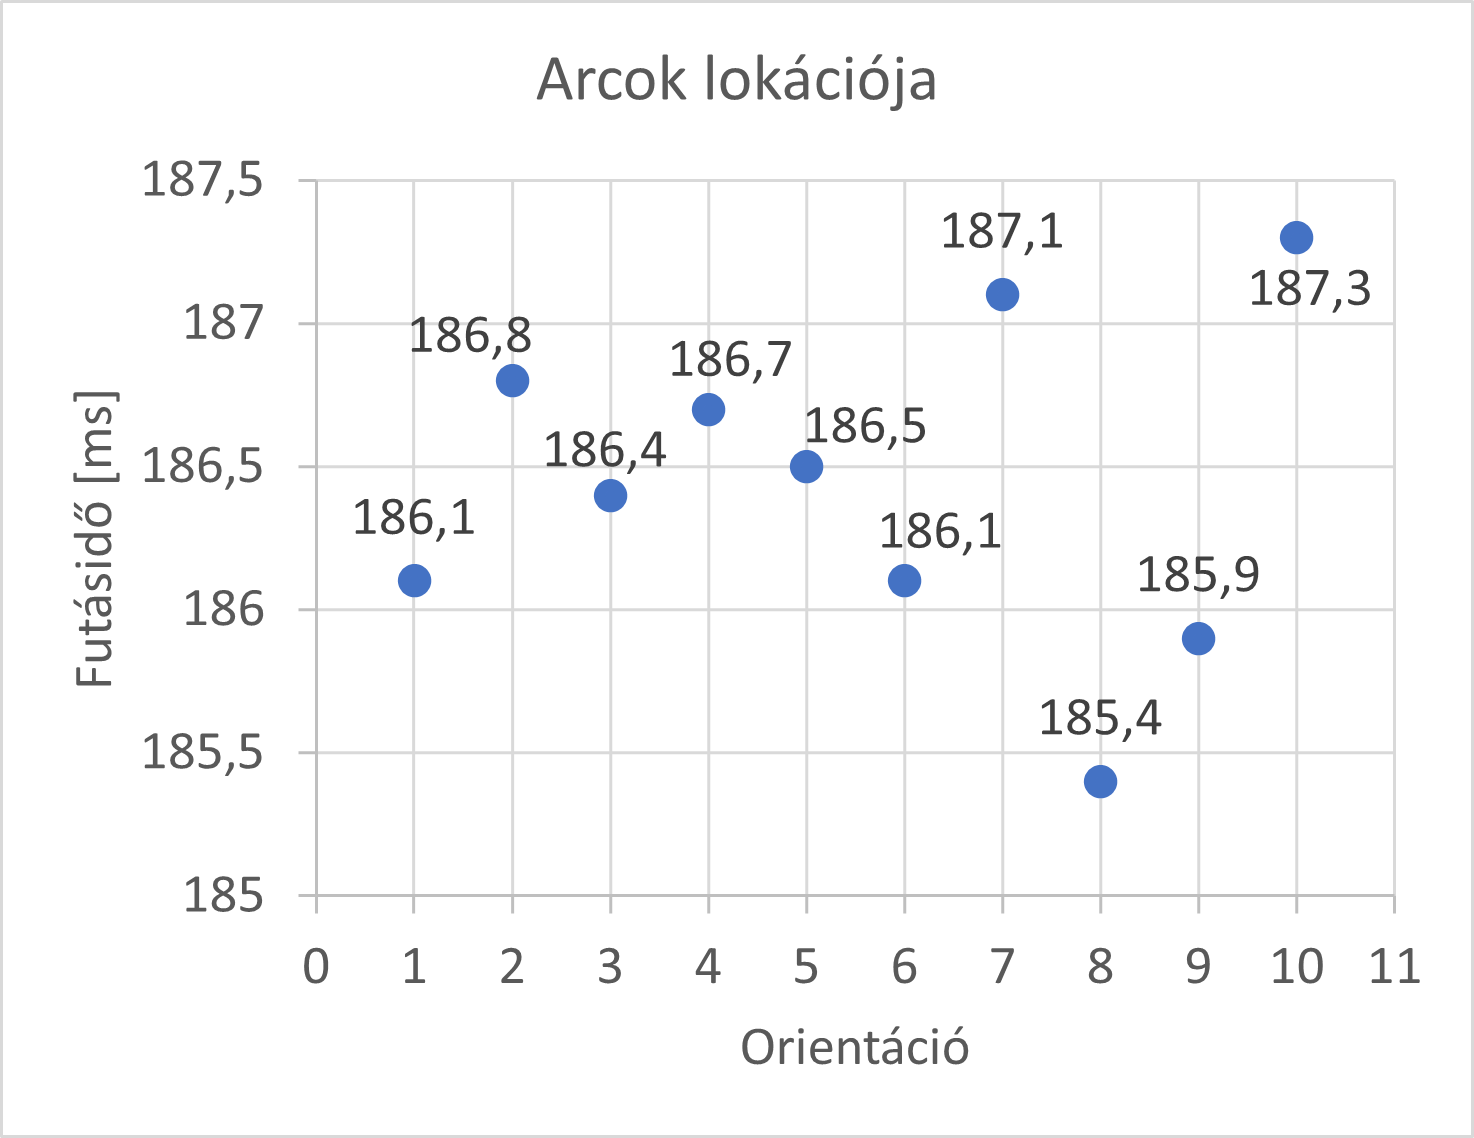
\includegraphics[width=67mm, keepaspectratio]{03_images/graph2/orientacio.png}\hspace{1cm}
	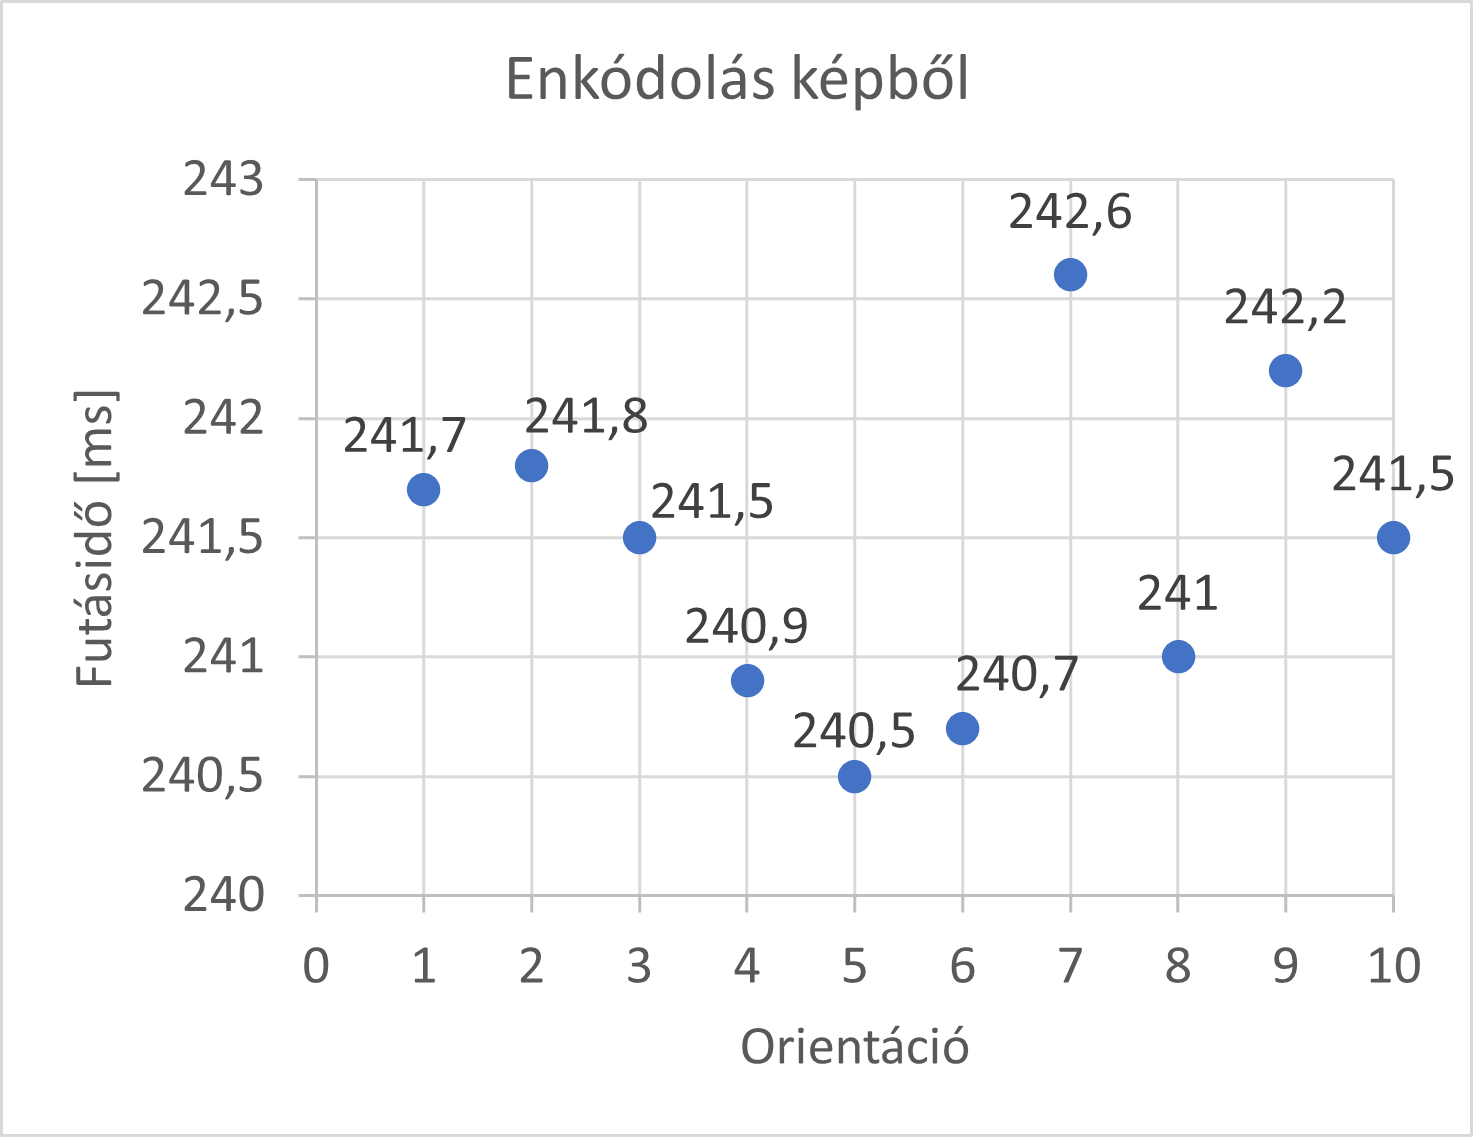
\includegraphics[width=67mm, keepaspectratio]{03_images/graph2/orientacio2.png}\\\vspace{5mm}
	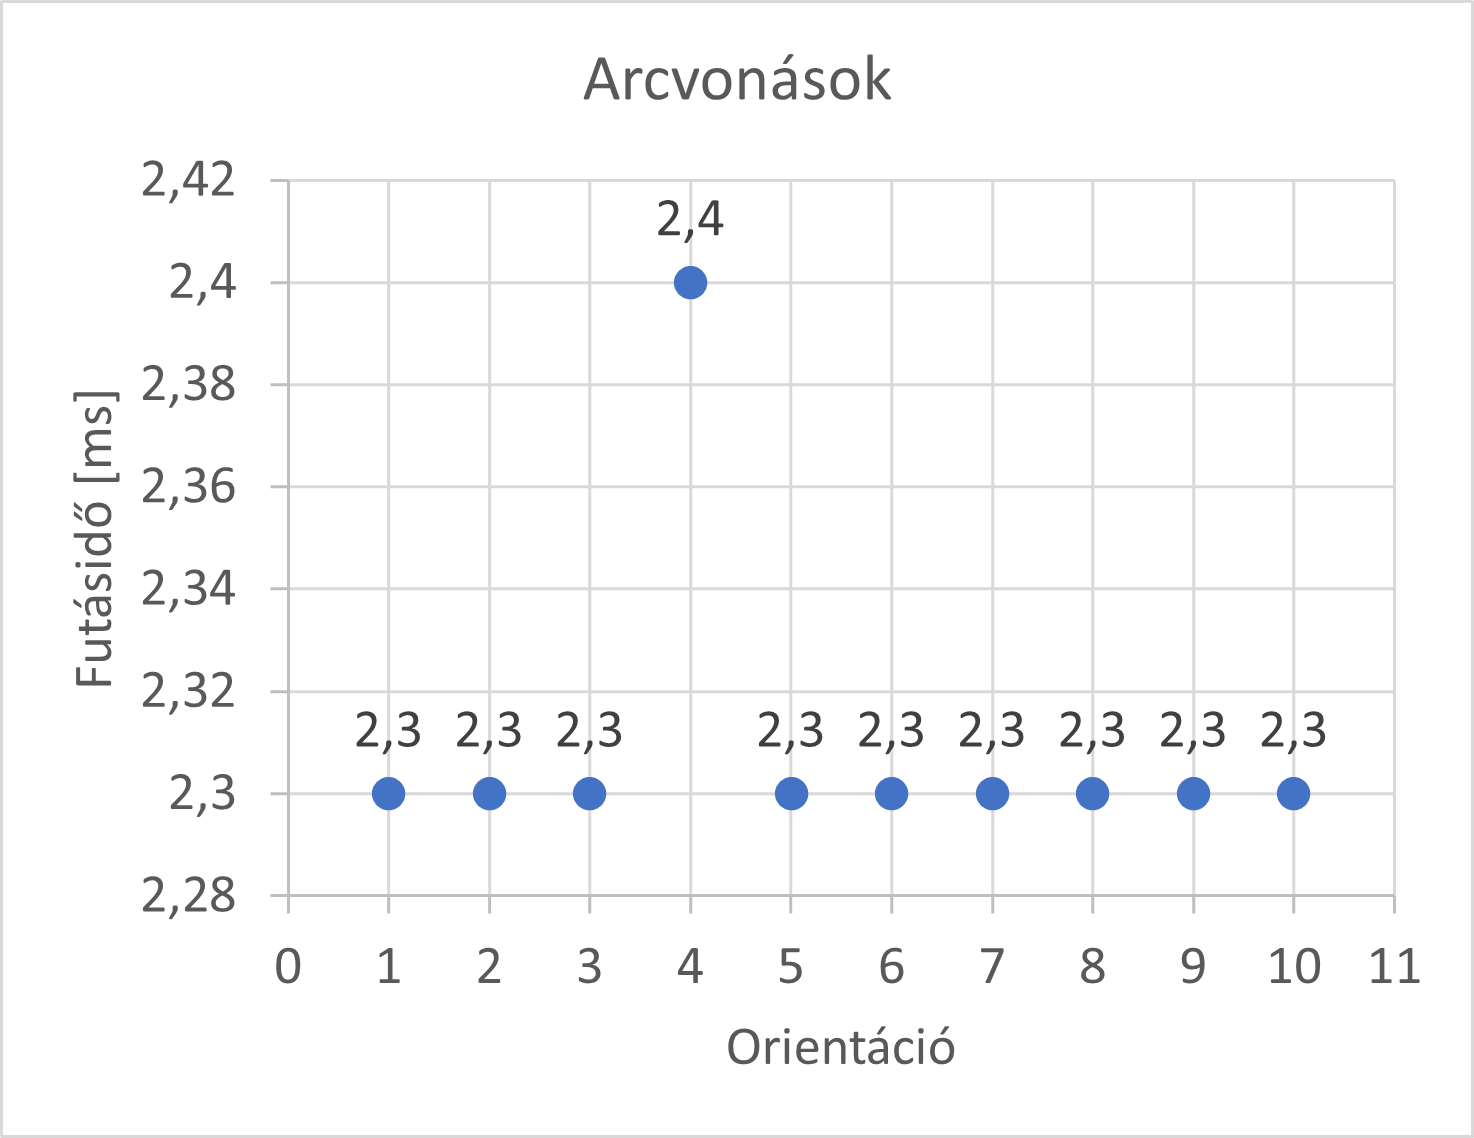
\includegraphics[width=67mm, keepaspectratio]{03_images/graph2/orientacio3.png}\hspace{1cm}
	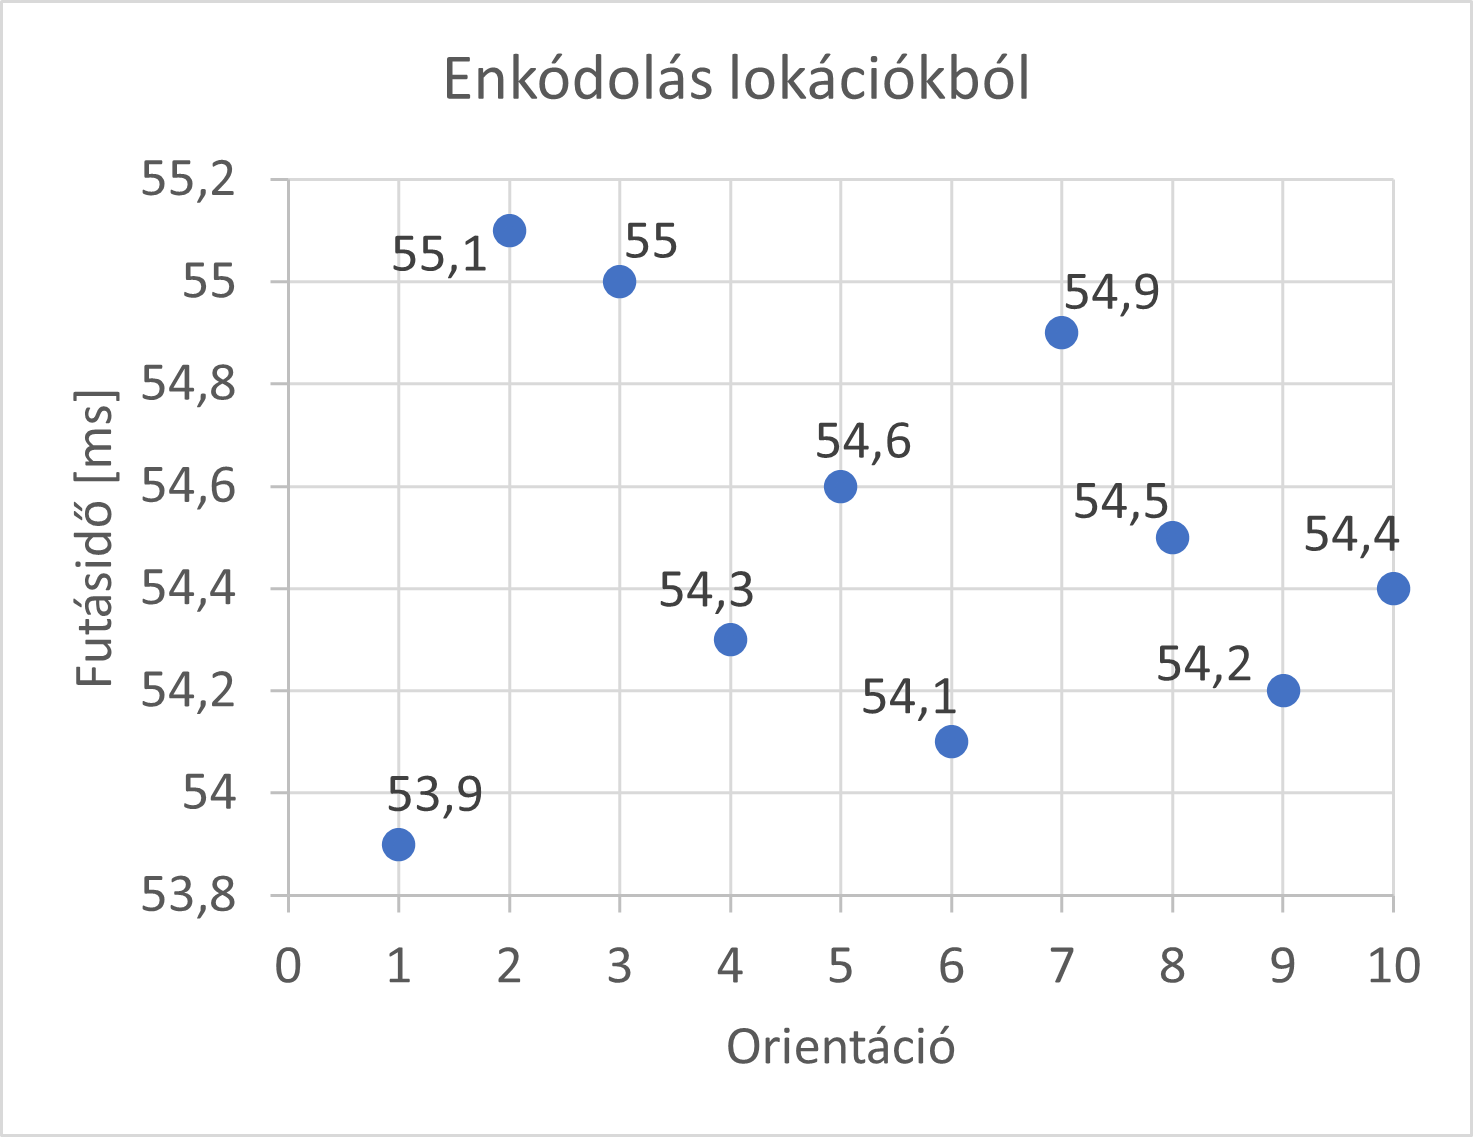
\includegraphics[width=67mm, keepaspectratio]{03_images/graph2/orientacio4.png}
	\caption{Grafikonok az orientáció teszt eredményeiről.}
	\label{fig:ori_graphs}
\end{figure}